	%% Copernicus Publications Manuscript Preparation Template for LaTeX Submissions
%% ---------------------------------
%% This template should be used for copernicus.cls
%% The class file and some style files are bundled in the Copernicus Latex Package, which can be downloaded from the different journal webpages.
%% For further assistance please contact Copernicus Publications at: production@copernicus.org
%% http://publications.copernicus.org/for_authors/manuscript_preparation.html


%% Please use the following documentclass and journal abbreviations for discussion papers and final revised papers.


%% 2-column papers and discussion papers
\documentclass[essd,discussion]{copernicus}

\begin{document}

\nocite{*}

\title{The AlborEx dataset: sampling of submesoscale features in the Alboran Sea}

\Author[1]{Charles}{Troupin}
\Author[2]{Ananda}{Pascual}
\Author[2]{Simon}{Ruiz}
\Author[3]{Antonio}{Olita}
\Author[2]{Benjamin}{Casas}
\Author[4]{Pierre-Marie}{Poulain}
\Author[5]{John~T.}{Allen}
\Author[6]{Amala}{Mahadevan}
\Author[5,2]{Joaqu\'{i}n}{Tintor\'{e}}

\affil[1]{GeoHydrodynamics and Environment Research, Freshwater and OCeanic science Unit of reSearch (FOCUS), University of Li\`{e}ge, Li\`{e}ge, Belgium}
\affil[2]{Instituto Mediterr\'{a}neo de Estudios Avanzados (IMEDEA, CSIC-UIB), Esporles, Spain}
\affil[3]{Institute for Coastal Marine Environment-National Research Council (IAMC-CNR) Oristano, Oristano, Italy}
\affil[4]{Istituto Nazionale di Oceanografia e di Geofisica Sperimentale (OGS), Trieste, Italy}
\affil[5]{Balearic Islands Coastal Observing and Forecasting System (SOCIB), Palma de Mallorca, Spain}
\affil[6]{Woods Hole Oceanographic Institution, Woods Hole, MA, USA}

\runningtitle{AlborEx database}
\runningauthor{Troupin et al.}
\correspondence{Charles Troupin (ctroupin@uliege.be)}

\received{}
\pubdiscuss{} %% only important for two-stage journals
\revised{}
\accepted{}
\published{}

%% These dates will be inserted by Copernicus Publications during the typesetting process.

\firstpage{1}

\maketitle


\begin{abstract}
AlborEx (Alboran Sea Experiment) consisted of a multi-platform, multi-disciplinary experiment performed in the Alboran Sea (Western Mediterranean Sea) between May 25 and 31, 2014. The observational component of the experiment focused on the sampling of the physical and biogeochemical properties of sea water within oceanographic features present along an intense frontal zone, with a particular interest in the resulting vertical motions. To this end, the mission included 1 research vessel (66 profiles), 2 underwater gliders (adding up 554 profiles), 3 Argo floats and 25 surface drifters. 

In addition, 500 water samples were collected at the 66 CTD stations for the measurement of chlorophyll and nutrient concentrations. Near real-time ADCP velocities were collected nightly and during the CTD sections. All of the Argo floats acquired temperature and conductivity profiles, while the Prov-bio float also measured oxygen and chlorophyll-a concentrations, colored dissolved organic matter, backscattering at 700 nm, downwelling irradiance at 380, 410, 490 nm, and photo-synthetically active radiation (PAR).

In the context of mesoscale and submesoscale interactions, the AlborEx dataset constitutes a particularly valuable source of information to infer mechanisms, evaluate vertical transport and establish relationships between the thermal and haline structures and the biogeochemical variable evolution, in a region characterised by strong horizontal gradients provoked by the confluence of Atlantic and Mediterranean Waters.

\end{abstract}


\introduction 

The variety of physical and biological processes occurring in the ocean at various spatial and temporal scales requires a combination of tools in order to properly understand the underlying mechanisms. Hydrodynamical models constitute such a tool: they make it possible to design specific numerical experiments or simulate idealised situation that can reproduce some of these processes and assess the impacts of climate change. Despite the continuous progresses made in modeling (spatial resolution, parameterization, atmospheric coupling, \ldots), in situ observations remain an essential yet challenging ingredient when addressing the complexity of the ocean. 

The perfect observational system would consist in dense array of sensors present at many geographical locations, many depths and measuring almost continuously a wide range of parameters. Obviously such a system is not the reality: researchers have to rely on the combination of various platforms during a limited period of time, each platform measuring a given set of variables at different spatial and temporal resolutions, spatial coverage, accuracy and depth levels. We will refer to this as multi-platform experiment, by opposition to experiments articulated only around the observations made using a research vessel. 

The western Mediterranean Sea is a particularly relevant region for multi-platform experiments, thanks to the wide range of processes taking place and intensively studied since the work of \citet{WUST61} on the vertical circulation: influence on climate \citep[e.g.,][]{GIORGI06,GIORGI08,ADLOFF15,GUIOT16,RAHMSTORF98} and sea-level change \citep[e.g.,][]{TSIMPLIS02, BONADUCE16,WOLFF18}, thermohaline circulation \citep[e.g.,]{BERGAMASCO10 MILLOT87,MILLOT91,MILLOT99,SKLIRIS14,ROBINSON01, water mass formation and convection process \citep[e.g.,]{STOMMEL72,SEND1999,MACIAS18}, mesoscale \citep[e.g.,][]{PUJOL05,SANCHEZROMAN17} and submesoscale processes.


The AlborEx multi-platform experiment was performed in the Alboran Sea from from May 25 to 31, 2014, with the objective of capturing meso and submesoscale processes taking place in this area and evaluating the interactions between the two scales, with a specific focus on the vertical velocities. The data set made up of the observations provided by all the platforms during that period, described in the next Section, is particularly rich data set due to the variety of sensors and measured variables concentrated on a relatively small area.

\section{The AlborEx mission}

The section aims to summarize the motivations behind the sampling and deployments. An extensive description of the available data is the object of the next section.

\subsection{Oceanographic context}

The particularity of the mission design is that the exact sampling area was not known until a few days before the start. Prior to the experiment, satellite images of sea surface temperature (SST) and chlorophyll-a (chl-a) concentration were acquired in order to provide an overview of the oceanic surface features visible in the Alboran Sea. A well-defined front (Fig.~\ref{fig1:SST}) separating Atlantic and Mediterranean waters and exhibiting filament-like structures was selected. 

The pair of images indicate that the front position barely changed between May 25 and 30, 2014. An anticyclonic eddy centered around 36$^{\circ}$30'N, 0.5$^{\circ}$W, according to altimetry data, slowly followed an eastward trajectory in the following days during the 

The description of features and processes occurring during the mission is not in the scope of this paper. The interested reader is invited to consult \cite{RUIZ2015} for a extensive description of the mission and \cite{PASCUAL2017} for the main findings deduced from the in-situ observations.

\begin{figure}[t]
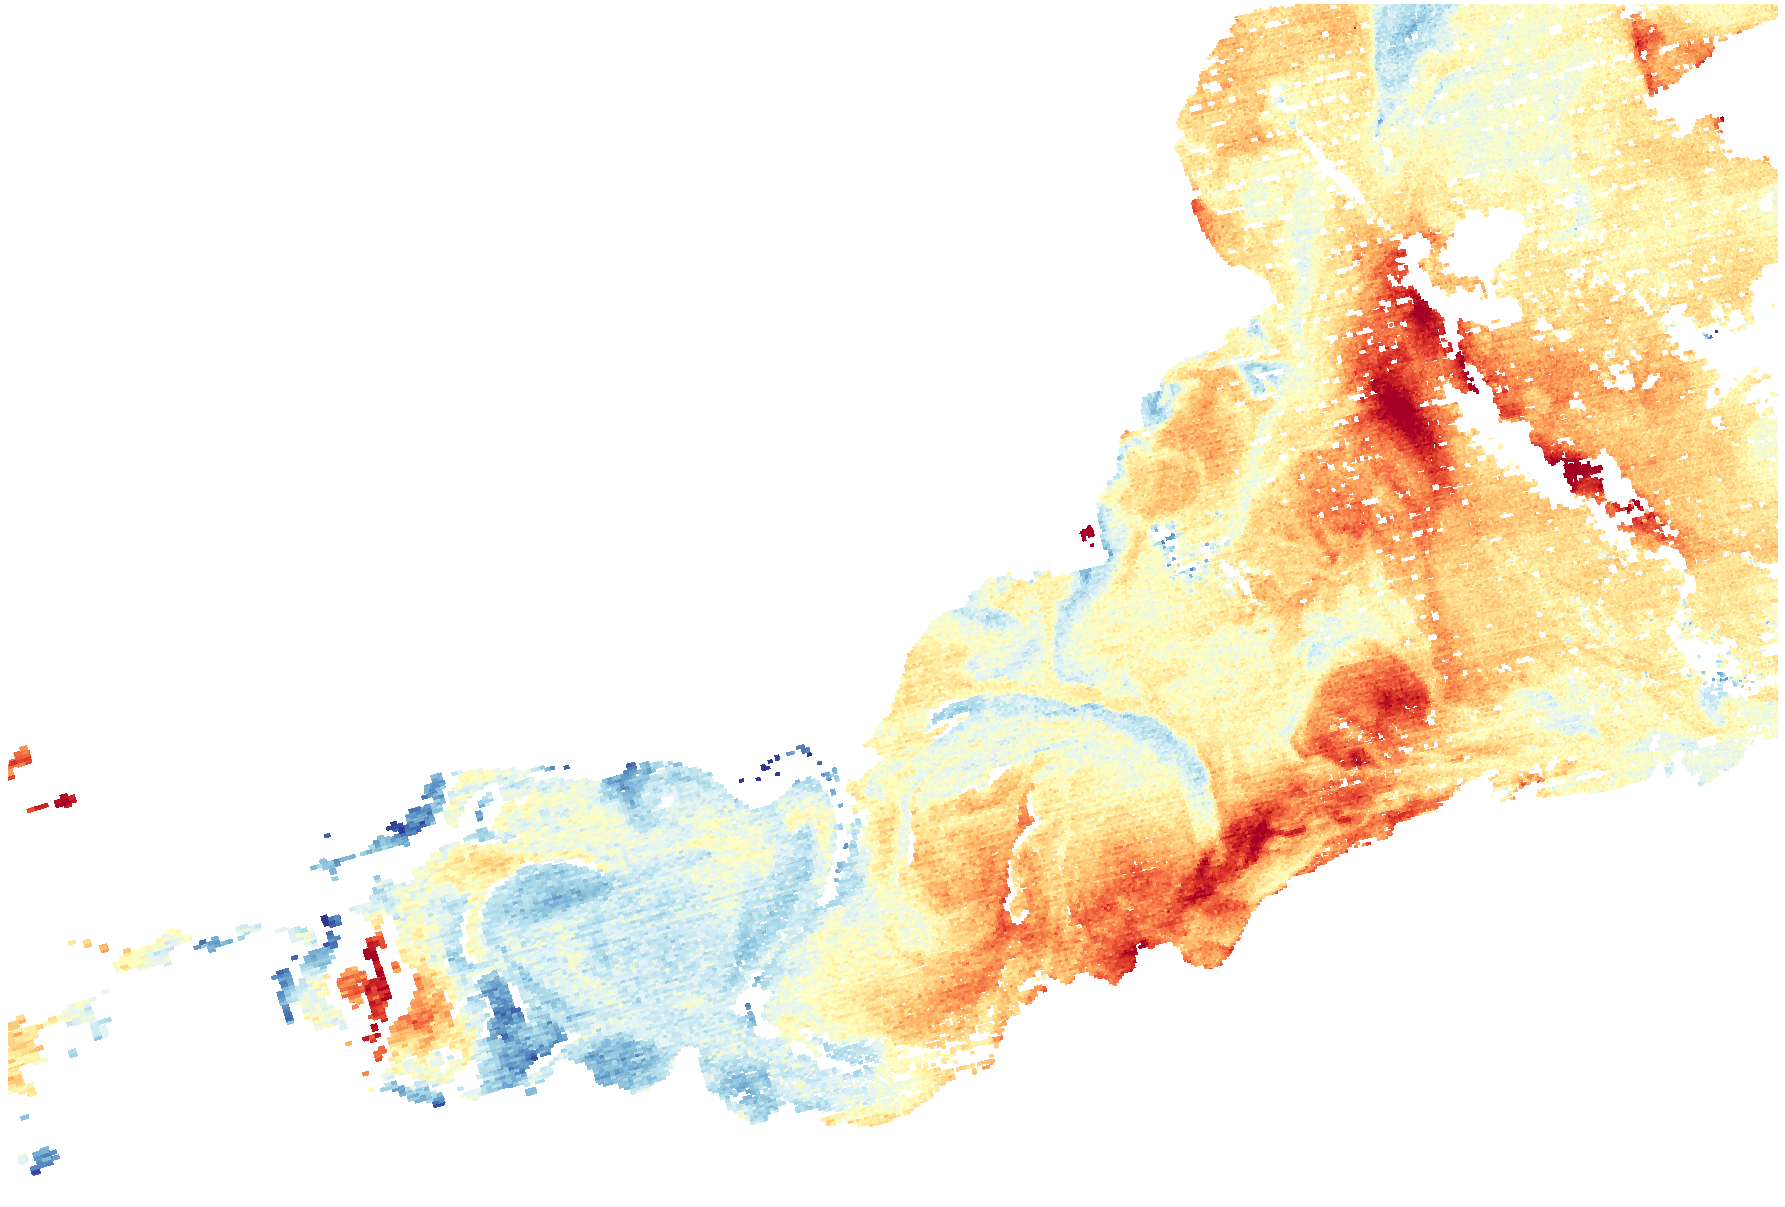
\includegraphics[width=.5\textwidth]{../figures/A2014145125000_L2_LAC_SST.png}\\
\includegraphics[width=.5\textwidth]{../figures/A2014150020500_L2_LAC_SST.png}
\caption{Sea Surface Temperature in the western Mediterranean Sea from MODIS sensor onboard Aqua Satellite corresponding to May 25 and 30, 2014. The dashed black line indicates the approximative position of the front. Level-2, 11 $\mu m$, night-time images were selected. Only pixels with a quality flag equal to 1 (good data) were represented.\label{fig1:SST}}
\end{figure}

\subsection{Sampling strategy}

While the remote sensing data represented a meaningful source of information about the front and the small scale features, in situ observation were essential to fulfill the mission objectives. Below are presented the different platforms deployed for the data collection.

\subsubsection{Research vessel}

The SOCIB R/V was used to sample the area with vertical profiles acquired though the CTD. Two distinct CTD surveys were performed on a 10~km $\times$ 5~km regular grid. The first survey was run from May 26 to 27 and consisted of 34 casts along 5 meridional legs (Fig.~\ref{fig2:CTD}). The second survey took place from May 29 to 30 and was made up of 28 casts. These casts were performed at almost similar locations as those of the first survey in order to allow for detecting changes between the two periods. 

\begin{figure}[t]
\includegraphics[width=.5\textwidth]{../figures/CTD/ctd_casts.png}
\caption{The CTD casts were organised in 5 legs that crossed the front and were repeated over 2 periods, at the beginning and the end of the mission.\label{fig2:CTD}}
\end{figure}

In addition to the CTDs, the R/V thermosalinograph continuously acquired temperature and conductivity along the ship track, from which near surface salinity is derived. Direct measurements of currents were performed during the night (from 10~PM UTC to 6~AM UTC) and during the 2 CTD surveys, using an acoustic Doppler current profiler (ADCP). The R/V weather station measured air temperature, pressure, wind speed and direction during the whole duration of the mission.

\begin{figure}[t]
\includegraphics[width=.5\textwidth]{../figures/CTD/ctd_casts.png}
\caption{The CTD casts were organised in 5 legs that crossed the front and were repeated over 2 periods, at the beginning and the end of the mission.\label{fig2:CTD}}
\end{figure}

\subsubsection{Gliders}

To collect measurements addressing the submesoscale, two gliders were deployed on May 25 inside the study area. The coastal glider carried out measurements up to 200~m depth  against 500~m for the deep glider. The horizontal resolution was about 0.5~km for the shallow and 1~km for the deep glider. The initial plan was to have two 50-km meridional tracks, 10 kilometers away one from the other, and to repeat these tracks up to 4 times during the experiment. However, due to the strong eastward currents, different tracks (Fig.~\ref{}) crossing the front several times were made instead.

On May 25, 25 Surface Velocity Program (SVP) drifters were deployed in the frontal area in a tight square pattern (mean distance between drifters around 3~km). Almost all the drifters also provided measurement of the sea water temperature near the surface. On the same day, three Argo floats were programmed to cycle	at intervals ranging from 3 hours to 5 days and to depths up to 2000~m.

\begin{figure}[t]
\includegraphics[width=.45\textwidth]{../figures/drifter_temperature.png}\includegraphics[width=.45\textwidth]{../figures/drifter_temperature_closeup.png}
\caption{Surface drifter trajectories. For the sake of simplicy the temperature, when available, is only shown for the duration of the mission.\label{fig3:drifters}}
\end{figure}

\section{Description of the database}

The AlborEx mission generated a large amount of data in a region scarcely sampled in the past. The synergy between lower-resolution (CTD, drifters) and high-resolution data (ADCP, gliders) makes this dataset unique for the study of submesoscale processes in the Mediterranean Sea. Moreover its multidisciplinary nature makes it suitable to study the interactions between the physical conditions and the biogeochemical variables.

\subsection{File format and organisation}

The original data files (i.e. obtained directly from the sensors) are converted to Network Common Data Form \citep[netCDF,][]{REW90}, an Open Geospatial Consortium (OGC) standard widely adopted in atmospheric and oceanic sciences. Each file contains the measurements acquired by the sensors as well the metadata (mission name, principal investigator, \ldots). The structure of the files follows the Climate and Forecast (CF) conventions \citep{DOMENICO13} and are based on the model of OceanSITES \citep{SEND2010}. 

\subsection{Data processing levels}

Several processing levels are defined for the data files, all of them are provided in the data set. The files are organized by \textit{deployments}, where a deployment is defined as an event initiated when an instrument is put at sea and finished once the instrument is recovered from sea. The following table summarizes the deployments performed during the experiment.

\begin{description}
\item[Level 0 (L0)]: this is the level closest to the original measurements, as it contains exactly the same data as the raw files provided by the instruments, but in a single file.
\item[Level 1 (L1)]: in this level, additional variables are derived from the existing ones (e.g., salinity, potential temperature). The attributes corresponding to each variable are stored in the netCDF file, with details of any modifications. Unit conversion are also applied if necessary.
\item[Level 2 (L2)]: this level consists of regular, homogeneous and instantaneous profiles obtained by interpolating the L1 data. It is only provided for gliders, mostly for visualization and post-processing purposes: specific tools designed to read and display profiler data can then be used the same way for gliders.
\end{description}

\begin{table*}[h]
\caption{Characteristics of the instrument deployments in AlborEx.}
\begin{tabular}{lcrrccc}
\tophline
Instruments 		& Number of deployments & Initial time	& Final time			& \multicolumn{3}{c}{Processing levels} \\
					& 						& 				& 						& L0 			& L1 		& L2 \\
\middlehline
Weather station on board R/V	& 1			& 2014-05-25	& 2014-05-02			& \checkmark	& \checkmark &  \\ 
ADCP on board R/V	& 1						& 2014-05-25	& 2014-05-02			& \checkmark	& \checkmark &  \\ 
CTD					& 1 (66 stations)		& 2014-05-25	& 2014-05-02			& \checkmark	& \checkmark &  \\ 
Gliders 			& 2						& 2014-05-25	& 2014-05-30 			& \checkmark 	& \checkmark & \checkmark \\
Surface drifters	& 25					& 2014-05-25	& beyond the experiment & \checkmark 	& \checkmark &  \\
Profiling drifters	& 3						& 2014-05-25	& beyond the experiment & \checkmark 	& \checkmark &  \\
\bottomhline
\end{tabular}
\belowtable{} % Table Footnotes
\end{table*}

\subsection{Quality control}

All of the data provided by SOCIB are applied quality checks to detect possibly wrong or suspect values. The two main exceptions are:
\begin{description}
\item[the gliders:] a set of quality checks have been added to the glider toolbox \citep{Troupin_2015}. 
\item[the CTD profiles:] new checks have been recently added to the processing chain.
\end{description}
As the new files will not be available before a full reprocessing of all the historical missions, we decided to provide the data files in their current state. A new version will be uploaded as soon as the processing has been performed.

\section{Data availability}

Following SOCIB general policy, the data are made available as netCDF files through the SOCIB Thematic Real-time Environmental Distributed Data Services (THREDDS) Data Server, a standard way to distribute metadata and data using a variety of remote data access protocols such as OPeNDAP (\url{https://www.opendap.org}), Web Map Service (WMS) or direct HTTP access. 

%Data are also available through the main European portals:
%\begin{itemize}
%\item Copernicus Marine Environment Monitoring Service (\url{http://marine.copernicus.eu/}), which  provides reference information on the state of the physical oceans and regional seas using numerical model and in situ observations.
%\item EMODnet Physics (\url{http://www.emodnet-physics.eu/}), an operational service gathering near real time and historical validated marine data in an interoperable way.
%\end{itemize}

However, none of the aforementioned solution allows users to get the whole data set in a common place. Hence the different files were submitted to the Zenodo research platform (\url{https://zenodo.org/}), which stores research outputs (papers, code, datasets) and assigns them a Digital Object Identifier (DOI) so to have them easily and uniquely citeable.


\conclusions[Conclusions and perspectives]

The AlborEx observations acquired in May 2014 constitutes a unique observational data set that captured mesoscale and submesocale features in a particularly energetic frontal zone in the western Mediterranean Sea. The potential uses of the dataset can be separated in different topics:
\begin{itemize}
\item Hydrodynamics model validation: but the timing and location of small-scale features 
\item High-resolution remote-sensing data validation: high quality in situ measurements of the sea surface are essential for the validation of operational product such SST or Ocean Color. 
\item Study of mechanisms: the Mediterranean Sea is often referred to as a laboratory for oceanography and in particular the Alboran Sea is the stage of intense processes of mixing, subduction and instabilities.
\item Assessment of mechanisms responsible for intense vertical motions.

\end{itemize} 

In the near future multi-platform, high-resolution missions will be critical for the validation of altimetric data acquired by SWOT mission from 2020 on. 



\authorcontribution{C.T. prepared the figures and the present manuscript.}

\competinginterests{The authors declare that the research was conducted in the absence of any commercial or financial relationships that could be construed as a potential conflict of interest.}

\disclaimer{The authors do not accept any liability for the correctness and appropriate interpretation of the data or their suitability for any use.}

\begin{acknowledgements}
The AlborEx experiment was conducted in the framework of PERSEUS EU-funded project (Grant agreement no: 287600). Glider operations were partially funded by JERICO FP7 project. AP acknowledges support from the Spanish National Research Program (E-MOTION/CTM2012-31014 and PRE-SWOT/CTM2016-78607-P). SR and AP are also supported by the Copernicus Marine Environment Monitoring Service (CMEMS) MedSUB project. EM is supported by a post-doctoral grant from the Conselleria d'Educaci\'{o}, Cultura i Universitats del Govern de les Illes Balears (Mallorca, Spain) and the European Social Fund. AC is a FNRS researcher under the FNRS BENTHOX project (Convention T.1009.15). The profiling floats and some drifters were contributed by the Argo-Italy program. The authors thank A.~Massanet, F.~Margirier, M.~Palmer, C.~Castilla and P.~Balaguer for their efficient work at sea and M.~Menna, G.~Notarstefano and A.~Bussani for their help with the drifter and float data processing.

%NASA Goddard Space Flight Center, Ocean Ecology Laboratory, Ocean Biology Processing Group. Moderate-resolution Imaging Spectroradiometer (MODIS) Terra Ocean Color Data; 2014 Reprocessing. %NASA OB.DAAC, Greenbelt, MD, USA. doi: \doi{10.5067/TERRA/MODIS_OC.2014.0}.
%Accessed on 03/07/2017



\end{acknowledgements}




%% REFERENCES

\bibliographystyle{copernicus}
\bibliography{Alborex2017ESSD.bib}
%%
%% URLs and DOIs can be entered in your BibTeX file as:
%%
%% URL = {http://www.xyz.org/~jones/idx_g.htm}
%% DOI = {10.5194/xyz}


%% LITERATURE CITATIONS
%%
%% command                        & example result
%% \citet{jones90}|               & Jones et al. (1990)
%% \citep{jones90}|               & (Jones et al., 1990)
%% \citep{jones90,jones93}|       & (Jones et al., 1990, 1993)
%% \citep[p.~32]{jones90}|        & (Jones et al., 1990, p.~32)
%% \citep[e.g.,][]{jones90}|      & (e.g., Jones et al., 1990)
%% \citep[e.g.,][p.~32]{jones90}| & (e.g., Jones et al., 1990, p.~32)
%% \citeauthor{jones90}|          & Jones et al.
%% \citeyear{jones90}|            & 1990



%% FIGURES

%% We suggest to put the figures in the correct order and placement within the text. This aids readability.
%% When figures and tables are placed at the end of the MS (article in one-column style), please add \clearpage
%% between bibliography and first table and/or figure as well as between each table and/or figure.


%% ONE-COLUMN FIGURES

%%f
%\begin{figure}[t]
%\includegraphics[width=8.3cm]{FILE NAME}
%\caption{TEXT}
%\end{figure}
%
%%% TWO-COLUMN FIGURES
%
%%f
%\begin{figure*}[t]
%\includegraphics[width=12cm]{FILE NAME}
%\caption{TEXT}
%\end{figure*}
%
%
%%% TABLES
%%%
%%% The different columns must be seperated with a & command and should
%%% end with \\ to identify the column brake.
%
%%% ONE-COLUMN TABLE
%
%%t
%\begin{table}[t]
%\caption{TEXT}
%\begin{tabular}{column = lcr}
%\tophline
%
%\middlehline
%
%\bottomhline
%\end{tabular}
%\belowtable{} % Table Footnotes
%\end{table}
%
%%% TWO-COLUMN TABLE
%
%%t
%\begin{table*}[t]
%\caption{TEXT}
%\begin{tabular}{column = lcr}
%\tophline
%
%\middlehline
%
%\bottomhline
%\end{tabular}
%\belowtable{} % Table Footnotes
%\end{table*}
%
%
%%% MATHEMATICAL EXPRESSIONS
%
%%% All papers typeset by Copernicus Publications follow the math typesetting regulations
%%% given by the IUPAC Green Book (IUPAC: Quantities, Units and Symbols in Physical Chemistry,
%%% 2nd Edn., Blackwell Science, available at: http://old.iupac.org/publications/books/gbook/green_book_2ed.pdf, 1993).
%%%
%%% Physical quantities/variables are typeset in italic font (t for time, T for Temperature)
%%% Indices which are not defined are typeset in italic font (x, y, z, a, b, c)
%%% Items/objects which are defined are typeset in roman font (Car A, Car B)
%%% Descriptions/specifications which are defined by itself are typeset in roman font (abs, rel, ref, tot, net, ice)
%%% Abbreviations from 2 letters are typeset in roman font (RH, LAI)
%%% Vectors are identified in bold italic font using \vec{x}
%%% Matrices are identified in bold roman font
%%% Multiplication signs are typeset using the LaTeX commands \times (for vector products, grids, and exponential notations) or \cdot
%%% The character * should not be applied as mutliplication sign
%
%
%%% EQUATIONS
%
%%% Single-row equation
%
%\begin{equation}
%
%\end{equation}
%
%%% Multiline equation
%
%\begin{align}
%& 3 + 5 = 8\\
%& 3 + 5 = 8\\
%& 3 + 5 = 8
%\end{align}
%
%
%%% MATRICES
%
%\begin{matrix}
%x & y & z\\
%x & y & z\\
%x & y & z\\
%\end{matrix}
%
%
%%% ALGORITHM
%
%\begin{algorithm}
%\caption{�}
%\label{a1}
%\begin{algorithmic}
%�
%\end{algorithmic}
%\end{algorithm}
%
%
%%% CHEMICAL FORMULAS AND REACTIONS
%
%%% For formulas embedded in the text, please use \chem{}
%
%%% The reaction environment creates labels including the letter R, i.e. (R1), (R2), etc.
%
%\begin{reaction}
%%% \rightarrow should be used for normal (one-way) chemical reactions
%%% \rightleftharpoons should be used for equilibria
%%% \leftrightarrow should be used for resonance structures
%\end{reaction}
%
%
%%% PHYSICAL UNITS
%%%
%%% Please use \unit{} and apply the exponential notation


\end{document}
